\chapter{Clase 10. Configuraciones geométricas}
\textbf{05/03/2025}

\section{Problemas p.14 del problemario}


\begin{minipage}[t]{0.48\textwidth}
    \noindent
    \begin{excercise}
        Tienes 9 puntos acomodados en 3 filas con 3 con tres puntos cada fila, formando un cuadrado. Sin levantar el lápiz, dibuja 4 segmentos de recta que pase por los 9 puntos.
    \end{excercise}
\end{minipage}
\begin{minipage}[t]{0.48\textwidth}
    \begin{center}
        \textbf{Solución}
    \end{center}
    \begin{center}
        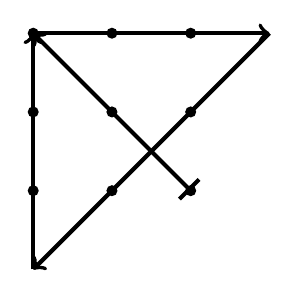
\begin{tikzpicture}[baseline=(current bounding box.north)]
    \fill (0,0) circle (2pt);
    \fill (0,1) circle (2pt);
    \fill (0,2) circle (2pt);

    \fill (1,0) circle (2pt);
    \fill (1,1) circle (2pt);
    \fill (1,2) circle (2pt);

    \fill (2,0) circle (2pt);
    \fill (2,1) circle (2pt);
    \fill (2,2) circle (2pt);

    %Linea que une los puntos
    \draw[line width=1.5,|->] (2,0) -- (0,2);
    \draw[line width=1.5,->] (0,2) -- (3,2);
    \draw[line width=1.5,->] (3,2) -- (0,-1);
    \draw[line width=1.5,->] (0,-1) -- (0,2);

\end{tikzpicture}


    \end{center}
\end{minipage}
\par

\bigskip
\noindent\hrule
\bigskip

\par
\begin{minipage}[t]{0.48\textwidth}
    \bigskip \bigskip
    \begin{excercise}
        Acomoda 9 puntos en 6 filas y cada fila con 3 puntos.
    \end{excercise}
\end{minipage}
\begin{minipage}[t]{0.48\textwidth}
    \noindent
    \begin{center}
        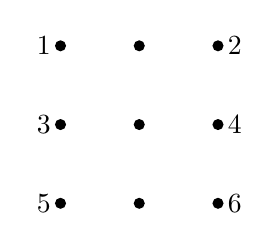
\begin{tikzpicture}[baseline=(current bounding box.north)]
    \fill (0,0) circle (2pt);
    \fill (0,1) circle (2pt);
    \fill (0,2) circle (2pt);

    \fill (1,0) circle (2pt);
    \fill (1,1) circle (2pt);
    \fill (1,2) circle (2pt);

    \fill (2,0) circle (2pt);
    \fill (2,1) circle (2pt);
    \fill (2,2) circle (2pt);

    % \etiquetas izquierda y derecha
    \node[left] at (0,2) {1};
    \node[right] at (2,2) {2};
    
    \node[left] at (0,1) {3};
    \node[right] at (2,1) {4};

    \node[left] at (0,0) {5};
    \node[right] at (2,0) {6};

\end{tikzpicture}


    \end{center}
    Si se ve de izquierda a derecha se tiene una fila, si se ve de derecha a izquierda es una fila distinta.
\end{minipage}
\par

\bigskip
\noindent\hrule
\bigskip

\par
\begin{minipage}[t]{0.48\textwidth}
    \begin{excercise}
        Acomoda 10 puntos en 5 filas y cada fila con 4 puntos.
    \end{excercise}
\end{minipage}
\begin{minipage}[t]{0.48\textwidth}
    \noindent
    \begin{center}
        \begin{tikzpicture}[baseline=(current bounding box.north)]
    % triangulo
    \fill[blue] (-1,2.5) circle (3pt);
    \fill[blue] (5,2.5) circle (3pt);
    \fill[blue] (2,1) circle (3pt);
    % punta de flecha
    \fill[blue] (0,0) circle (3pt);
    \fill[blue] (2,4) circle (3pt);
    \fill[blue] (4,0) circle (3pt);

    % nombramos las lineas de la estrella de 5 puntos
    \draw[name path=linea1, line width=1.5pt] (0,0) -- (2,4);
    \draw[name path=linea2, line width=1.5pt] (0,0) -- (5,2.5);
    \draw[name path=linea3, line width=1.5pt] (4,0) -- (-1,2.5);
    \draw[name path=linea4, line width=1.5pt] (4,0) -- (2,4);
    \draw[name path=linea5, line width=1.5pt] (-1,2.5) -- (5,2.5);

    % nombrando las intersecciones de las lineas
    \path[name intersections={of=linea1 and linea3, by={A}}];
    \path[name intersections={of=linea1 and linea5, by={B}}];
    \path[name intersections={of=linea2 and linea3, by={C}}];
    \path[name intersections={of=linea2 and linea4, by={D}}];
    \path[name intersections={of=linea4 and linea5, by={E}}];
    
    % marcando las intersecciones    
    \fill[blue] (A) circle (3pt);
    \fill[blue] (B) circle (3pt);
    \fill[blue] (C) circle (3pt);
    \fill[blue] (D) circle (3pt);
    \fill[blue] (E) circle (3pt);

\end{tikzpicture}

    \end{center}
\end{minipage}
